\chapter{Additional Pipeline Information}
\section{Derivations of the Flow Variance}
\label{sec:derivation_flow_var}
Flow estimation can be noisy for various reasons and the problem is that the nois is often proportional to the magnitude of the absolud flow. thus using a simple flow difference as ameasure will constantly underestimate the simmilarity between heigh magnitude flow. Hence, let us assume 
\begin{equation}
\begin{aligned}
\colvec{u_1}{v_1} = f + \colvec{x_1}{y_1} \\
\colvec{u_2}{v_2} = f + \colvec{x_2}{y_2}
\end{aligned}
\label{eq:def_flow_tracking}	
\end{equation}

where f is the true flow and 
\begin{equation}
	\colvec{x_1}{y_1} \sim \colvec{x_2}{y_2}
\end{equation}

Let us assume, that the random variables $x_1$ and $x_2$ are i.i.d. distributed having a zero mean and a variance $\sigma_x^2$, $x_1$ and $x_2$ respectively, i.e.

\begin{equation}
\begin{aligned}
x_1 \sim x_2 (0, \sigma_x^2) \\
y_1 \sim y_2 (0, \sigma_y^2
\end{aligned}
\label{eq:def_flow_tracking}	
\end{equation}

\begin{equation}
\begin{aligned}
\mathbf{E} \left[ \norm{\colvec{u_1}{v_1} - \colvec{u_2}{v_2}} \right]
& = \mathbf{E} \left[ (u_1 - u_2)^2 \right] + \mathbf{E} \left[ (v_1 - v_2)^2 \right] \\
& = \mathbf{E} \left[ u_1^2 - 2 u_1 u_2 + u_2^2 \right] + \mathbf{E} \left[ v_1^2 - 2 v_1 v_2 + v_2^2 \right] \\
& = \mathbf{E} \left[ x_1^2 \right] + \mathbf{E} \left[ x_2^2 \right] + \mathbf{E} \left[ y_1^2 \right] + \mathbf{E} \left[ y_2^2 \right] \\
& = 2 \left( \sigma_x^2 + \sigma_y^2 \right)
\end{aligned}
\label{eq:flow_variance_formula}	
\end{equation}
In the last step of Equation $\ref{eq:flow_variance_formula}$ we used the abbreviation $\sigma_x^2$ which denotes the variance of the optical flow along its $x$ direction. In this derivation we exploited the fact that $x_1$ and $x_2$ are independent random variables, $y_1$ and $y_2$ respectively. Hence, the term $\mathbf{E} \left[ x_1 x_2\right]$ yields the value zero. \\ \\
We experimentally also have defined an expression for computing depth variances. However, we this special run-mode has only been implemented to demonstrate the limitations of our pipeline. Therefore, the description of this procedure can be found in the appendix in Section $\ref{sec:depth_field_variances}$ on page $\pageref{sec:depth_field_variances}$.

\chapter{Additional Theoretical Background}
\section{On Filtering Images}
\subsection{Gaussian Filter}
A Gaussian filter (\textbf{GF}) is a linear operator that reduces noise by smoothing the image. Applying GF corresponds to a low-pass filtering.
At each position it estimates a local average of the intensities as defined in Equation $\ref{eq:gaussian_filtering_def}$.
\begin{equation}
	\mathcal{F}^{\text{gf}} \{I \} (p) = \sum_{q \in \Omega_p} G_{\sigma} (\norm{p - q}) I_q
\label{eq:gaussian_filtering_def}
\end{equation}
where $I$ defines the input image and $\Omega_p$ contains all neighboring points within the window that are centered at the image point $p$. Moreover, $G_{\sigma}$ denotes the two dimensional Gaussian kernel, which is defined in Equation $\ref{eq:def_g_weight}$.
\begin{equation}
	G_{\sigma} (x) = \frac{1}{2 \pi \sigma^2} e^{-\frac{x^2}{2 \sigma^2}}
\label{eq:def_g_weight}
\end{equation}
The Gaussian filtering is the weighted average of the intensity of the adjacent positions with a weight decreasing with the spatial distance to the center position. This distance is defined by $G_{\sigma} (\norm{p - q})$ where $\sigma$ is a parameter that defines the size of the neighborhood. The resulting image is a blurred version of the input image.

\subsection{Bilateral Filter}
\label{sec:bilateral_filter}
A Bilateral filter (\textbf{BF}) is a non-linear operator that reduces noise by smoothing the image but at the same time preserves its edges. \\ \\
The rational of this filter is that two pixels are close to each other if not only if their spacial distance is small but also if they are similar regarding their intensity range.
\begin{figure}[H]
\begin{center}
\subfigure[Raw Image]{
   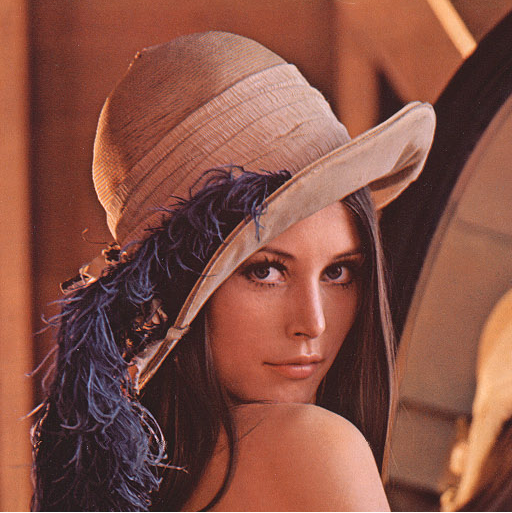
\includegraphics[width=0.47\linewidth] {background/filtering/l_raw}
}
\subfigure[Filtered Image]{
   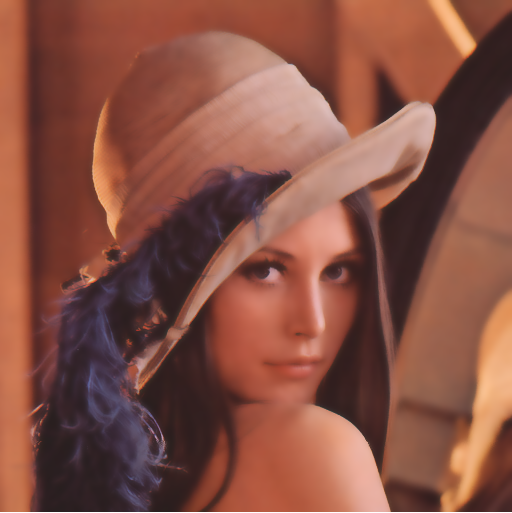
\includegraphics[width=0.47\linewidth] {background/filtering/l_filtered}
}
\end{center}
\caption[Example Bilateral Filter]{A bilateral filtering example: On the left side a noisy input image on the right its bilateral filtered version.}
\label{fig:bilat_filtering_eg}
\end{figure}
The filter replaces the intensity values at each pixel in an image by a weighted average of intensity values from nearby pixels. In our formulation we rely on the Gaussian distributions $G$ for defining the weights. Crucially, the weights depend not only on distances between pixels, but also on the intensity difference. That is why, when iterating through each pixel and adjusting weights to the adjacent pixels accordingly, Sharp edges are preserved. A bilateral filtering example$\footnote{All illustrated results were generated by using our own Bilateral filter implementation. For further information please visit our repository at \url{https://github.com/simplay/master_thesis}}$ is shown in Figure $\ref{fig:bilat_filtering_eg}$.\\ \\
The mathematical definition of this filter is given in Equation $\ref{eq:def_bilateral_filter}$. For a given Image $I$ we want to compute its bilateral filtered version by applying the following definition:
\begin{equation}
\begin{aligned}
&\mathcal{F}^{\text{bf}} \{I \} (p) = \frac{1}{W_p} \sum_{q \in \Omega_p} \underbrace{G_{\sigma_s} (\norm{p-q})G_{\sigma_r} (I_p - I_q)}_{w_p} I_q \\	
& \text{where } W_p = \sum_{q \in \Omega_p} G_{\sigma_s} (\norm{p-q})G_{\sigma_r} (I_p - I_q)
\end{aligned}
\label{eq:def_bilateral_filter}
\end{equation}
The set $\Omega_p$ contains all neighboring points within the window that are centered at the image point $p$. The scalar $W_p$ denotes the normalization factor of the filter and $I_p$ represents the image intensity at the pixel position $p$. Please notice that the definition of the bilateral filter is given per pixel, i.e. gives an representation of the filtered pixel intensity. \\ \\
The bilateral filter is controlled by the two parameters $\sigma_s$ and $\sigma_r$. The range variance increases $\sigma_r$, the BF becomes closer to the Gaussian blur filter. In other words, the larger $\sigma_r$ the more weight a pixel with a large intensity deviation gets. However, when increasing the spatial variance $\sigma_s$ results in smoothing larger features, i.e more distant pixels get a larger weight and thus influence the result more. Figure $\ref{fig:bfilter_influence_sigmas}$ demonstrates the influence of these parameters.
\begin{figure}[H]
\begin{center}
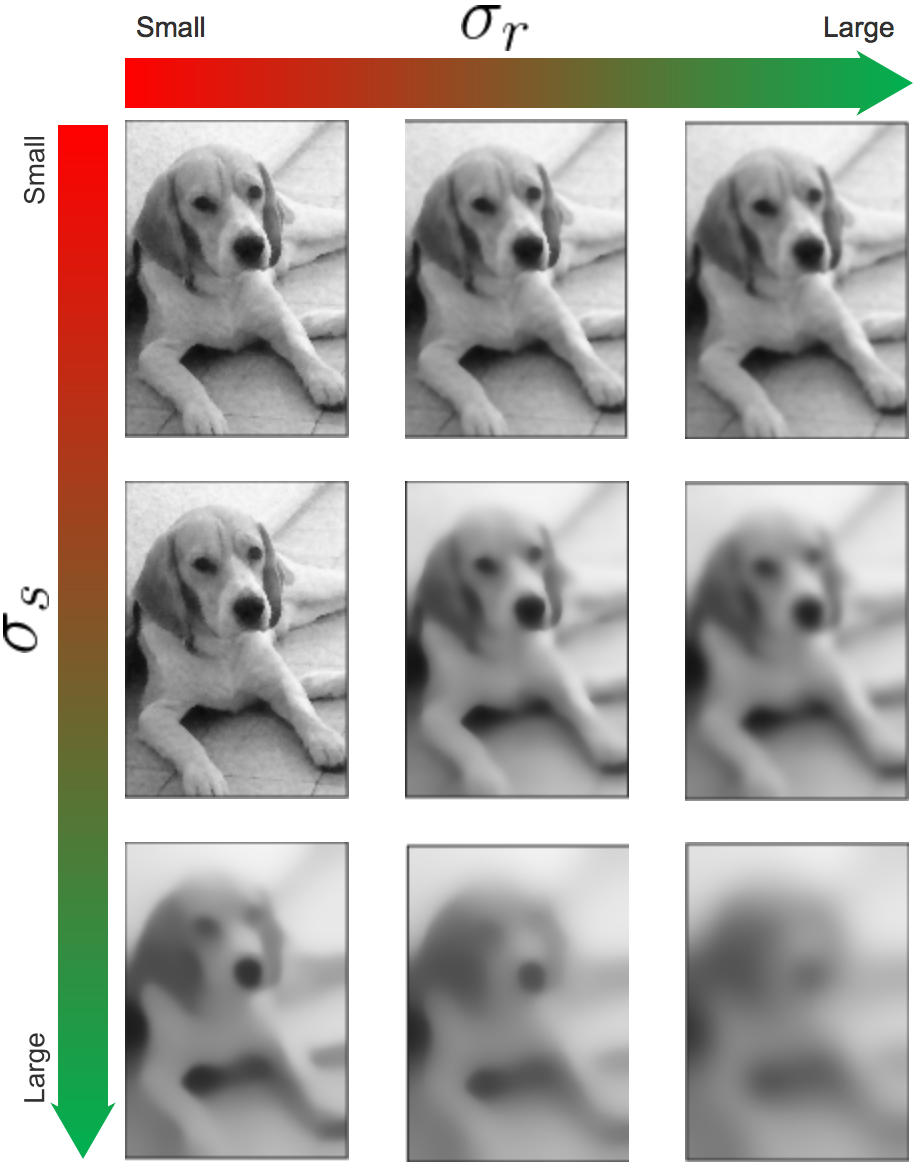
\includegraphics[width=0.6\linewidth] {background/filtering/bilat_filter_sigmas}
\end{center}
\caption[Influence of $\sigma_s$ and $\sigma_r$]{Different filtering results produced by our bilateral filter implementation for varying $\sigma_s$ and $\sigma_r$ values.}
\label{fig:bfilter_influence_sigmas}
\end{figure}

\subsection{Harris Corner Detector}
\label{sec:harris_corner_detector}
In this section we explain the principles of the Harris corner detector $\cite{Harris88acombined}$. Let us, therefore, consider a grayscale image $I$. We are going to sweep a window $w(x,y)$ (with displacements u in the x direction and v in the right direction) I and will calculate the variation of intensity. Since we are looking for windows with corners, we are looking for windows with a large variation in intensity. Hence, we have to maximize the equation above, specifically the term:
\begin{equation}
	E \left( u, v \right) = \sum_{x,y} w \left( x,y \right) \left[ I(x + u, y + v) - I(x, y) \right]^2
\label{eq:var_intensitiy_def}
\end{equation}
Next, the term $I(x + u, y + v)$ is expressed by the first order taylor series expansion as the follows:
\begin{equation}
	I(x + u, y + v) = I(x,y) + u I_x (x, y) + v I_y (x,y) + \text{h.o.t}
\label{eq:taylor_exp_intensity}
\end{equation}
Next, we put the first order approximation of Equation $\ref{eq:taylor_exp_intensity}$ into Equation $\ref{eq:var_intensitiy_def}$ to simplify the definition of $E$.
\begin{equation}
\begin{aligned}
E \left( u, v \right) 
&= \sum_{x,y} w \left( x,y \right) \left[ I(x + u, y + v) - I(x, y) \right]^2 \\
&\approx \sum_{x,y} w \left( x,y \right) \left[ I(x,y) + u I_x (x, y) + v I_y (x,y) - I(x, y) \right]^2 \\
&= \sum_{x,y} w \left( x,y \right) \left[ u I_x (x, y) + v I_y (x,y) \right]^2 \\
&= \sum_{x,y} w \left( x,y \right) u^2 I_x^2 + 2 u v I_x I_y v^2 I_y^2 \\
&= \left( u,v \right) \left( \sum_{x,y} w (x,y)
\begin{pmatrix}
I_x^2 & I_x I_y \\
I_x I_y & I_y^2 \\
\end{pmatrix}
\right) \colvec{u}{v}
\end{aligned}
\label{eq:var_intensitiy_developed}
\end{equation}
Let us define the following substitution
\begin{equation}
M = \sum_{x,y} w  (x,y)
\begin{pmatrix}
I_x^2 & I_x I_y \\
I_y^2 & I_x I_y \\
\end{pmatrix}
\label{eq:var_intensity_sub}
\end{equation}
Putting the substitution from Equation $\ref{eq:var_intensity_sub}$ into the final form of Equation $\ref{eq:var_intensitiy_developed}$ we obtain the final form
\begin{equation}
	E \left( u, v \right) \approx \left( u,v \right) M \colvec{u}{v}
\end{equation}.
A score is calculated for each window, to determine if it can possibly contain a corner:
\begin{equation}
\begin{aligned}
& R = \det(M) - \kappa \left(\text{trace}(M)\right)^2 \\
&\text{where } \det(M) = \lambda_1 \lambda_2 \text{ and } \text{trace}(M) = \lambda_1 + \lambda_2
\end{aligned}
\label{eq:harris_response}
\end{equation}

\section{On Statistics}
\label{sec:on_statistics_bg}

\subsection{Conditional Probability}
Given two events $A$ and $B$ with the probability $P(B) > 0$. The conidtional probability of $A$ given $B$ is defined as
\begin{equation}
	P(A|B) = \frac{P(A \cap B)}{P(B)}
\label{eq:conditional_prob}
\end{equation}
Furthermore, Equation $\ref{eq:conditional_prob}$ gives us an alternative interpretation of the probability of an intersection
\begin{equation}
P(A \cap B) = P(A|B)P(B) 	
\end{equation}
The probability that two events happen the same time is the same as the Probability of the event A given B times the probability of event B. Sticking to this definition, we can visualize all possible outcomes of two events happening the same time as shown in Figure $\ref{fig:prob_tree_diagram}$.
\begin{figure}[H]
\begin{center}
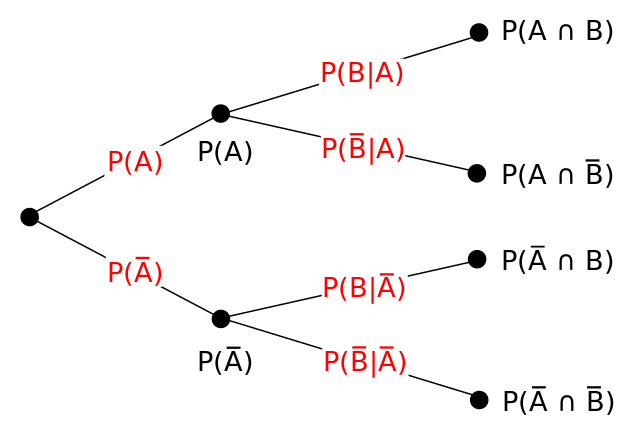
\includegraphics[width=0.45\linewidth] {background/statistics/probability_tree_diagram}
\end{center}
\caption[Probability Tree Diagram]{Tree liked representation$\footnotemark$ of the four possible outcomes for a conditional probability.}
\label{fig:prob_tree_diagram}
\end{figure}
\footnotetext{The visualized graphic has been taken from: \url{https://en.wikipedia.org/wiki/File:Probability_tree_diagram.svg}}



\subsection{Evaluating Binary Classifiers}
In this section we explain the mathematical framework we use in our evaluation.


The purpose of a binary classifier is to classify given elements into two groups according to a specified classification rule. Think about a binary random variable modelling a certain event. The actual observations of the random variable are then either equals true or false. A classification$\footnote{I.e. the produced output after applying the classifier on the given data.}$ of a given dataset yields two numbers: the number of the positives and negatives, which add up to the size of the set. \\ \\
In order to evaluate the quality of binary classifier its prediction is compared against a standard reference method or, if existing, against a ground truth assignment and then cross tabulates the data into a $2 \times 2$ contingency table as shown in Figure $\ref{tab:prediction_sensitivity}$. 
\begin{table}[H]
\centering
\begin{tabular}{c|c|c|}
\cline{2-3}
 & \begin{tabular}[c]{@{}l@{}}Prediction\\ Positive\end{tabular} & \begin{tabular}[c]{@{}l@{}}Prediction\\ Negative\end{tabular} \\ \hline
\multicolumn{1}{|l|}{\begin{tabular}[c]{@{}l@{}}Condition\\ Positive\end{tabular}} & \cellcolor[HTML]{34FF34}{\color[HTML]{000000} $\bf{TP}$ } & \cellcolor[HTML]{CB0000} $\bf{FN}$ \\ \hline
\multicolumn{1}{|l|}{\begin{tabular}[c]{@{}l@{}}Condiation\\ Negative\end{tabular}} & \cellcolor[HTML]{CB0000}{\color[HTML]{000000} $\bf{FP}$ } & \cellcolor[HTML]{34FF34} $\bf{TN}$ \\ \hline
\end{tabular}
\caption[Conditional Probability]{The four possible outcomes of a conditional probability}
\label{tab:prediction_sensitivity}
\end{table}
There are four possible outcomes: the classifier prediction, which has either are positive or negative condition, was actually correct or incorrect. \\ \\
Let us consider the following example where we test some people for the presence of a disease. Some of these people have the disease, and the test correctly detects them. These findings are called true positives (\textbf{TP}). Some have the disease, but the test incorrectly claims that they do not have it. These results are called false negatives (\textbf{FN}). Some people do not suffer from the disease and the test classifies correctly as health. These results are called true negatives (\textbf{TN}). And Lastly, some healthy people who are incorrectly classified as infected. These are the so called false positives (\textbf{FP}) results. \\ \\
There are many metrics that can be used to measure the performance of a classifier. In the following a listing of some prominent metrics
%
\begin{itemize}
\item \textbf{Precision}: Tells us what proportion of patients we diagnosed as having the disease actually had that disease. In other words, proportion of TP in the set of positive disease diagnoses. This is given by the rightmost column in the confusion matrix.
\begin{equation}
	\text{precision} = \frac{\text{TP}}{\text{TP} + \text{FP}}
\label{eq:def_precision}
\end{equation}
\item \textbf{Recall}: Tells us what proportion of people that actually had the disease were diagnosed by the test as having the disease. In other words, proportion of TP in the set of true disease states. This is given by the bottom row in the confusion matrix.
\begin{equation}
	\text{recall} = \frac{\text{TP}}{\text{TP} + \text{FN}}
\label{eq:def_recall}
\end{equation}
\end{itemize}
A visualization of these measures is given in Figure $\ref{fig:eval_concept_recall_precc}$.
\begin{figure}[H]
\begin{center}
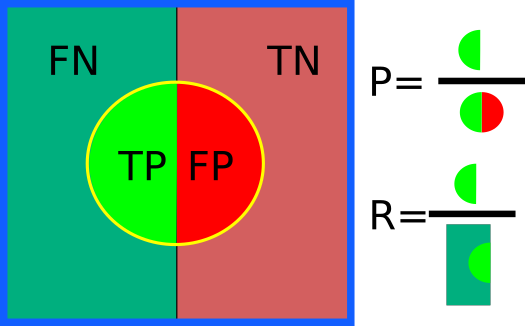
\includegraphics[width=0.6\linewidth] {evaluation/prec_recall}
\end{center}
\caption[Concept Recall and Precision]{This figure illustrates graphically the concept of Recall (\textbf{R}) and Precision (\textbf{P}). When estimating the sampling of a binary random variable, there are basically four possible outcomes: The we predicted it being true and it is true (\textbf{TP}), we predicted it true but it is false (\textbf{FP}), we predicted it false and it was actually negative (\textbf{FN}) or we predicted it to be true but it was actually false (\textbf{TN}). }
\label{fig:eval_concept_recall_precc}
\end{figure}
An alternative measure is the $F_1$ score. This measure is often used in determining the performance of classification tasks in machine learning. To compute its score, this measure takes into account both, the precision and the recall of the test. The exact definition of the F1 measure is given in Equation $\ref{eq:f1_score}$.
\begin{equation}
F_1 = 2 \left( \frac{\text{precision} \times \text{recall}}{\text{precision} +\text{recall}} \right)
\label{eq:f1_score}
\end{equation}  
The F1 score can be interpreted as a normalized weighted average of the precision and recall measures. The best possible F1 score is equals 1 and its worst value is 0.

\section{Camera Model}
\subsection{Pinhole Camera}
\label{sec:pinhole_camera}
A camera projects a 3d scene in a 2d image. A simple mathematical model to describe such a mapping from the 3d scene space to the 2d image space is the pinhole camera model. This model is conceptually illustrated in Figure $\ref{fig:pinhole_camera_model}$.
\begin{figure}[H]
\begin{center}
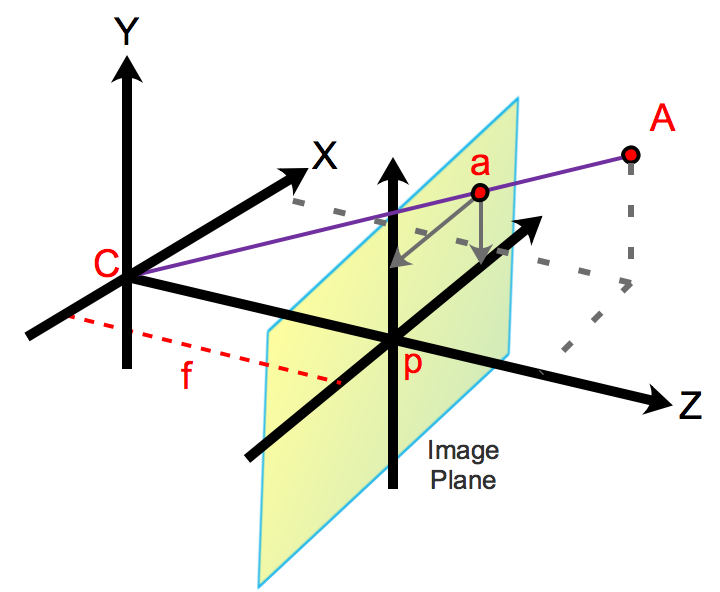
\includegraphics[width=0.8\linewidth] {background/camera_model/pinhole_camera}
\end{center}
\caption[Pinhole Camera Model]{Visualizing the pinhole camera model. The camera center $C$ represents an infinitely small aperture hole and assumed to be located at $(0,0,0)$, $f$ is the focal length in pixel units, $p$ is the principal point in images coordinates, $\textbf{A} = (X, Y, Z)$ a 3d point in the scene and $\textbf{a} = (f \frac{X}{Z}, f \frac{Y}{Z})$ its projected pixel version mapped onto the image plane.}
\label{fig:pinhole_camera_model}
\end{figure}
The aperture is an infinitely small hole and there is no lens used to focus light. Therefore, lens distorting or depth of field effects are ignored. The intersection point where all rays meet is the center of the perspective projection and usually referred by \textit{camera center}. The principal axis is formed by the line perpendicular to the image plane, which passes though the camera center. Its intersection point with the image plane is called principal point. The distance between the camera center and the principal point is the so called focal length.

\subsection{Camera Parameters}
\paragraph{Intrinsic Parameters} Let $\textbf{X} = (X,Y,Z,1)^T$ denote a point in a 3D scene and $\textbf{x} = (x,y,1)^T$ its projected version in the image plane. Both points are written in their homogeneous form. The mapping from a scene point to the image plane is defined as
\begin{equation}
\textbf{x} = 
\begin{pmatrix}
f & s & p_x & 0 \\
0 & f & p_y & 0 \\
0 & 0 & 1 & 0
\end{pmatrix}
\textbf{X}
\end{equation}
where $f$ denotes the focal length and $p = (p_x, p_y)^T$ the offset to the origin in image coordinates with respect to the principal point. In modern cameras, the skew $s$ is usually equals zero. The parameters $f$, $p_x$, $p_y$ and $s$ are called \textit{intrinsic camera parameters}. Notice, that $\textbf{X}$ is expressed in terms of camera coordinates and similarly, $\textbf{x}$ in pixel coordinates.

\paragraph{Extrinsic Parameters} In general, a camera is not located at the origin of the world coordinate system and can have an arbitrary orientation. Let $\textbf{X}_w$ denote a point, living in an arbitrary camera coordinate system. To express this point in the regular camera coordinate system, we have to apply a certain transformation. In a rigid object model, the points $\textbf{X}$ and $\textbf{X}_w$ can be transformed to one another by applying a linear transformation that consists of a rotational matrix $R$ and a translation $t$. The actual mapping is defined as
\begin{equation}
	X = \left[ R | t \right] X_w
\end{equation}
The parameters $t$ and $R$ are called \textit{extrinsic camera parameters}.


%% ADDITIONAL EXPERIMENTS
\chapter{Additional Experiment and Statistics}
In this appendix chapter we put a series of extra experiments as well as all numeric measurements not previously shown in the results chapter.

\section{Additional Experiment: Varying CC/EV}
\label{sec:additional_cc_ev_exp}
In this experiment we examine the bahaviour of LDOF PED MC method for a varying the eigenvalue-cluster count. For 2 to 6 clusters and for 2 to 6 eigenvectors we generate segmentations on the Waving Hand dataset and plot the resulting performance (Fig. $\ref{fig:wh_altering_ev_cc_app}$. This experiment will give us some further insight about choosing appropriate eigenvalue (EV) and cluster count (CC) we want to solve for in MinCut (MC) and Spectral clustering (SC). The corresponding statistics are listed in Table $\ref{tab:wh_ev_c}$. To give the reader a easier way to understand the results we visualized the resulting statistics. For fixed cluster counts, we plotted the recall-precession and the eigenvector-f1 score graphs. Moreover, for fixed eigenvector counts we plotted the resulting recall-precession and clusters-f1 score graphs. 
\begin{figure}[H]
\begin{center}
\subfigure[Varying Clusters Recall/Precision Plot]{
   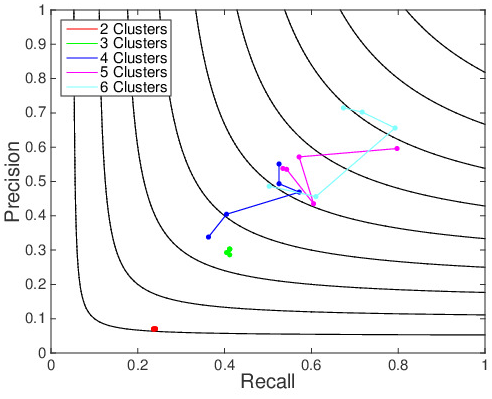
\includegraphics[width=0.47\linewidth] {evaluation/wh1/perf_ev_c/clusters_rec_prec}
}
\subfigure[Varying Clusters EV/F1 Score Plot]{
   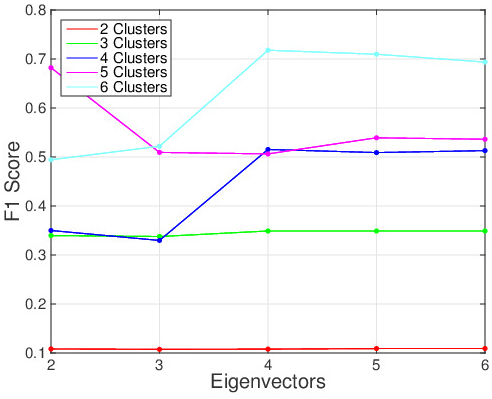
\includegraphics[width=0.47\linewidth] {evaluation/wh1/perf_ev_c/clusters_ev_f1}
}
\subfigure[Varying EV Recall/Precision Plot]{
   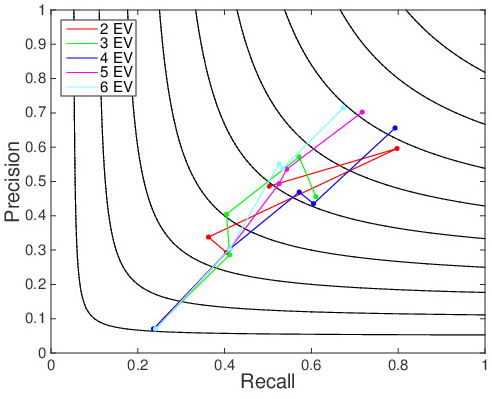
\includegraphics[width=0.47\linewidth] {evaluation/wh1/perf_ev_c/ev_rec_prec}
}
\subfigure[Varying EV Clusters/F1 Score Plot]{
   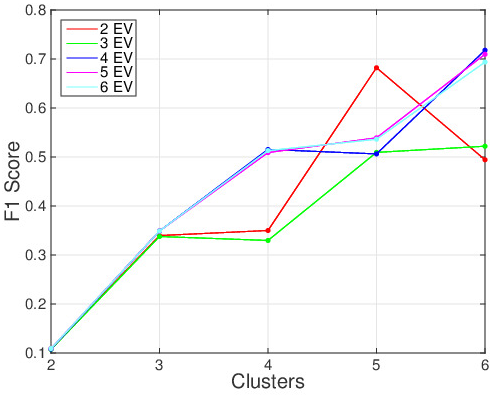
\includegraphics[width=0.47\linewidth] {evaluation/wh1/perf_ev_c/ev_c_f1}
}
\end{center}
\caption[Plot Performance Varying CLusters/Eigenvectors]{Visualizing the experiment \enquote{Varying CC/EV} via graphs: For a fixed number of eigenvectors and an altering cluster count (first row) we show the recall/precision and eigenvector/F1-Score plots. Similarly, we show recall/precision and clusters/F1-Score plots plots for a fixed number of clusters and an altering number of eigenvectors (second row). The utilized measurements for this plots is listed in Table $\ref{fig:wh_altering_ev_cc_app}$.}
\label{fig:wh_altering_ev_cc_app}
\end{figure}

\begin{table}[H]
\centering
\begin{tabular}{|l|c|c|c|c|c|}
\hline
\multicolumn{6}{|c|}{Performance Varying Eigenvectors/Clusters PED MC} \\ \hline
\multicolumn{6}{|c|}{Precision} \\ \hline
\textbf{Eigenvectors / Clusters} & 2 & 3 & 4 & 5 & 6 \\ \hline
2 & 7.03\% & 29.28\% & 33.80\% & 59.61\% & 48.63\%  \\ \hline
3 & 6.95\% & 28.62\% & 40.45\% & 57.17\% & 45.59\%  \\ \hline
4 & 6.99\% & 30.28\% & 46.90\% & 43.53\% & 65.60\%  \\ \hline
5 & 7.05\% & 30.28\% & 49.35\% & 53.55\% & 70.23\%  \\ \hline
6 & 7.05\% & 30.28\% & 50.11\% & 53.81\% & 71.47\%  \\ \hline
\multicolumn{6}{|c|}{Recall} \\ \hline
2 & 23.64\% & 40.45\% & 36.28\% & 79.73\% & 50.27\%  \\ \hline
3 & 23.64\% & 41.17\% & 40.45\% & 57.17\% & 61.04\%  \\ \hline
4 & 23.64\% & 41.17\% & 57.20\% & 60.50\% & 79.28\%  \\ \hline
5 & 24.09\% & 41.17\% & 52.55\% & 54.29\% & 71.71\%  \\ \hline
6 & 24.09\% & 41.17\% & 52.55\% & 53.42\% & 67.39\%  \\ \hline
\multicolumn{6}{|c|}{F1 Score} \\ \hline
2 & 10.83\% & 33.97\% & 35.00\% & 68.22\% & 49.43\%  \\ \hline
3 & 10.74\% & 33.77\% & 32.97\% & 50.94\% & 52.20\%  \\ \hline
4 & 10.79\% & 34.90\% & 51.54\% & 50.63\% & 71.79\%  \\ \hline
5 & 10.91\% & 34.90\% & 50.90\% & 53.92\% & 70.97\%  \\ \hline
6 & 10.91\% & 34.90\% & 51.30\% & 53.62\% & 69.37\%  \\ \hline
\end{tabular}
\caption[Performance Varying Eigenvector-Cluster]{Measurements of the experiment \enquote{Varying CC/EV} on the Waving Hand dataset (Fig. $\ref{fig:wh_altering_ev_cc_app}$).}
\label{tab:wh_ev_c}
\end{table}

\section{Varying Cluster Count on SC and MC}
This experiment should examine the behaviour of the modes PD SC, PD MC, PED SC, PED MC when using LDOF flow fields for a varying number of clusters on the One Chair dataset (Fig. $\ref{fig:chair_3_cast_dataset_appendix}$). The quantitative results are visualized in Figure $\ref{fig:chair_3_cast_plot_avg_stat}$. Additionally, qualitative results of the best resulting segmentations (Fig. $\ref{fig:chair_3_cast_best_f_score_results}$) and the worst result (Fig. $\ref{fig:chair_3_cast_gt_worst_best}$) are visualized below. The corresponding measurements of these experiments are listed in Table $\ref{tab:chair_3_cast_avg_performance}$.
\begin{figure}[H]
\begin{center}
\subfigure[Frame 30]{
   \includegraphics[width=0.31\linewidth] {evaluation/chairs_3_cast/ds/45}
}
\subfigure[Frame 45]{
   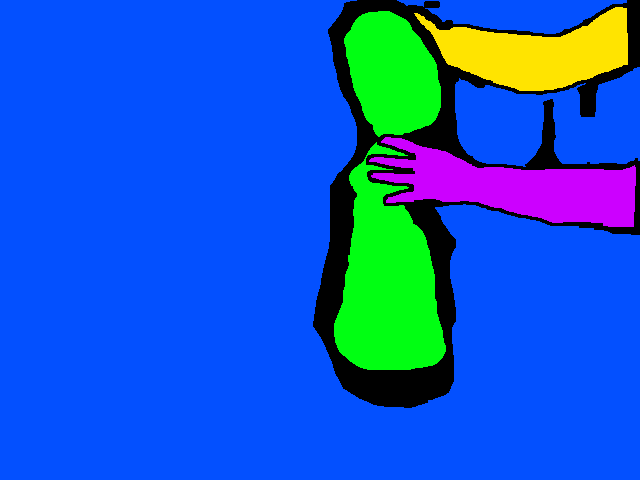
\includegraphics[width=0.31\linewidth] {evaluation/chairs_3_cast/ds/60}
}
\subfigure[Frame 60]{
   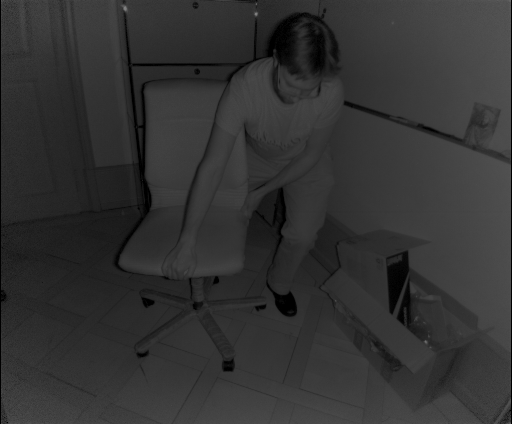
\includegraphics[width=0.31\linewidth] {evaluation/chairs_3_cast/ds/75}
}
~
\subfigure[Gt Frame 45]{
   \includegraphics[width=0.31\linewidth] {evaluation/chairs_3_cast/gt/45}
}
\subfigure[GT Frame 60]{
   \includegraphics[width=0.31\linewidth] {evaluation/chairs_3_cast/gt/60_amb}
}
\subfigure[GT Frame 75]{
   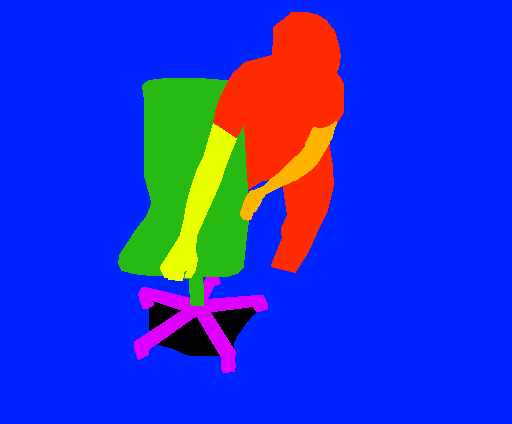
\includegraphics[width=0.31\linewidth] {evaluation/chairs_3_cast/gt/75_amb}
}
\end{center}
\caption[Chair 3 Cast Dataset]{Visualizing the ground truth frame and their frames of the One Chairs dataset}
\label{fig:chair_3_cast_dataset_appendix}
\end{figure}

\begin{figure}[H]
\begin{center}

\subfigure[Raw 5 Clusters PED MC]{
   \includegraphics[width=0.22\linewidth] {evaluation/chairs_3_cast/best/ped_mc_c_5}
}
\subfigure[5 Clusters PED MC]{
   \includegraphics[width=0.22\linewidth] {evaluation/chairs_3_cast/merged/ped_mc_c_5}
}
\subfigure[Raw 10 Clusters PED MC]{
   \includegraphics[width=0.22\linewidth] {evaluation/chairs_3_cast/best/ped_mc_c_10}
}
\subfigure[10 Clusters PED MC]{
   \includegraphics[width=0.22\linewidth] {evaluation/chairs_3_cast/merged/ped_mc_c_10}
}
~
\subfigure[Raw 15 Clusters PD SC]{
   \includegraphics[width=0.22\linewidth] {evaluation/chairs_3_cast/best/pd_sc_c_15}
}
\subfigure[15 Clusters PD SC]{
   \includegraphics[width=0.22\linewidth] {evaluation/chairs_3_cast/merged/pd_sc_c_15}
}
\subfigure[Raw 20 Clusters PD SC]{
   \includegraphics[width=0.22\linewidth] {evaluation/chairs_3_cast/best/ped_mc_c_20}
}
\subfigure[20 Clusters PED MC]{
   \includegraphics[width=0.22\linewidth] {evaluation/chairs_3_cast/merged/ped_mc_c_20}
}
\end{center}
\caption[Chair 3 Cast Winner]{Listing the four top segmentation results of frame 60 according to their scored F1 value (Tab. $\ref{tab:chair_3_cast_avg_performance})$. On the left, the unmerged- and on the right the merged segmentation.}
\label{fig:chair_3_cast_best_f_score_results}
\end{figure}

\begin{table}[H]
\centering
\begin{tabular}{|l|c|c|c|c|}
\hline
\multicolumn{5}{|c|}{Average Precision} \\ \hline
\textbf{Method / \#Cluster} & 5 & 10 & 15 & 20 \\ \hline
PD SC & 18.01\% & \textbf{55.17}\% & \textbf{55.12}\% & \textbf{56.23}\% \\ \hline
PD MC & \textbf{38.70}\% & 38.14\% & 45.65\% & 49.64\% \\ \hline
PED SC & 13.14\% & 35.29\% & 50.75\% & 52.14\%  \\ \hline
PED MC & 26.81\% & 42.94\% & 38.70\% & \textbf{56.23}\% \\ \hline
\multicolumn{5}{|c|}{Average Recall} \\ \hline
PD SC & 12.34\% & 19.22\% & 38.13\% & 47.82\% \\ \hline
PD MC & 13.10\% & 24.51\% & \textbf{44.07}\% & \textbf{53.50}\% \\ \hline
PED SC & 10.20\% & 28.29\% & 39.24\% & 33.75\% \\ \hline
PED MC & \textbf{19.37}\% & \textbf{38.86}\% & 41.88\% & 50.07\% \\ \hline
\multicolumn{5}{|c|}{Average F1 Score} \\ \hline
PD SC & 14.02\% & 28.47\% & \textbf{45.04}\% & 51.59\% \\ \hline
PD MC & 19.50\% & 29.79\% & 44.63\% & 51.40\% \\ \hline
PED SC & 11.48\% & 30.89\% & 43.88\% & 40.69\% \\ \hline
PED MC & \textbf{21.97}\% & \textbf{40.63}\% & 40.12\% & \textbf{52.58}\% \\ \hline
\end{tabular}
\caption[Chair 3 Cast: Average Precision Scores]{Average results of the experiment \enquote{varying number of clusters} on the One Chair dataset.}
\label{tab:chair_3_cast_avg_performance}
\end{table}

\begin{figure}[H]
\begin{center}

\subfigure[Recall / Precision Plot]{
   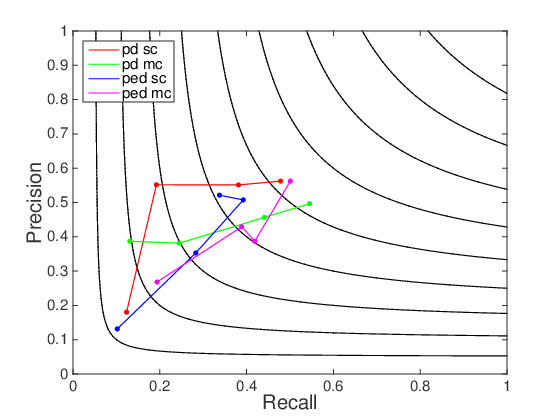
\includegraphics[width=0.47\linewidth] {evaluation/chairs_3_cast/avg/avg_prec_rec}
   \label{fig:chair_3_cast_plot_avg_stat_a}
}
\subfigure[Cluster Count / F1 Score Plot]{
   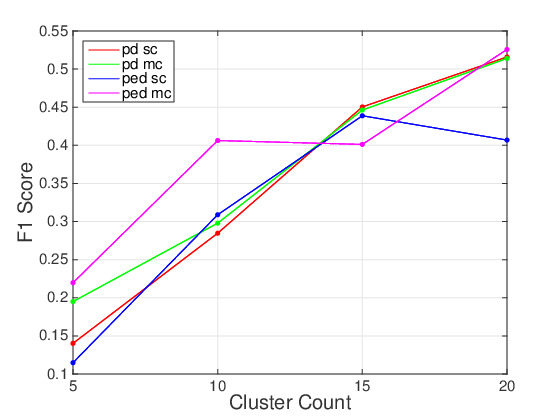
\includegraphics[width=0.47\linewidth] {evaluation/chairs_3_cast/avg/avg_clust_f1}
   \label{fig:chair_3_cast_plot_avg_stat_b}
}
\end{center}
\caption[Chair 3 Cast avg statistic plots]{Plots of the average performance of the four methods PED SC, PD MC, PED SC and PED MC for a varying number of clusters. The left plots shows the recall/precision plot and the figure on the right shows the F1 score alongside the number of clusters. The actual measurements are listed in Table $\ref{tab:chair_3_cast_avg_performance}$.}
\label{fig:chair_3_cast_plot_avg_stat}
\end{figure}

\begin{figure}[H]
\begin{center}
\subfigure[Ground truth frame 60]{
   \includegraphics[width=0.31\linewidth] {evaluation/chairs_3_cast/worst_best/60_amb}
   \label{fig:chair_3_cast_gt_worst_best_a}
}
\subfigure[Worst F1 Score Frame 60]{
   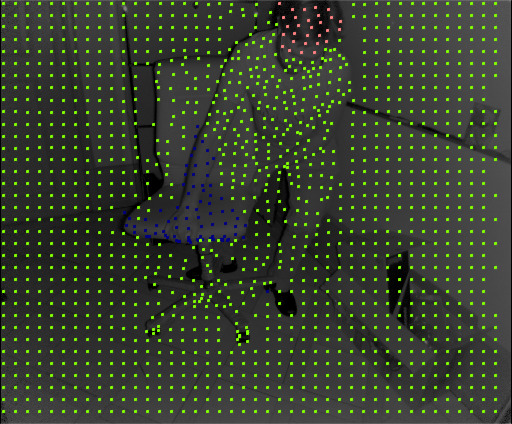
\includegraphics[width=0.31\linewidth] {evaluation/chairs_3_cast/worst_best/ped_sc_c_5_f_60}
   \label{fig:chair_3_cast_gt_worst_best_b}
}
\subfigure[Best F1 Score Frame 60]{
   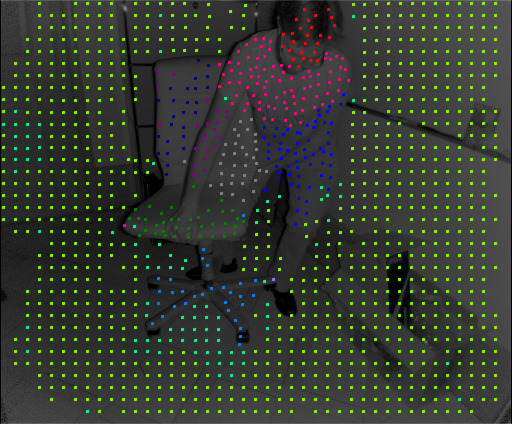
\includegraphics[width=0.31\linewidth] {evaluation/chairs_3_cast/worst_best/ped_mc_c_20_f_60}
   \label{fig:chair_3_cast_gt_worst_best_c}
}
\end{center}
\caption[Chair 3 Cast Worst/Best Result]{Comparison of the worst- (center) and the best (right) segmentation results according to the F1 measure (see Tab. $\ref{tab:chair_3_cast_avg_performance}$) using the shown mask on the left.}
\label{fig:chair_3_cast_gt_worst_best}
\end{figure}